\documentclass[letterpaper,12pt]{article}
\usepackage[margin=1in]{geometry}
\usepackage{libertine}
\usepackage{parskip}
\usepackage{graphicx}
\pagestyle{empty}
\begin{document}

\hspace*{-1in}

\includegraphics[scale=0.9]{CoverPage.jpg}

\title{Two Graph Vertex Partitioning Algorithms for Part Consolidation in Axiomatic Design}
\author{Jeffery Cavallaro}
\date{15 August 2019}
\maketitle
\section*{Abstract}
In traditional manufacturing, parts are designed and manufactured separately so that the parts can be combined into
subassemblies, which are then combined into final assemblies.  Indeed, the standardization of parts was one of the
key developments that fueled the explosive growth of manufacturing during the \(19^{th}\) and \(20^{th}\)
centuries.  Now, in the \(21^{st}\) century, a new technique, referred to as \emph{additive manufacturing},
promises a new leap forward in manufacturing capability: instead of manufacturing the parts for subassemblies
separately, the subassemblies are constructed directly through the additive application of layers of material,
commonly referred to as \emph{3-D printing}.

But what is the best way to allocate parts into subassemblies in order to minimize the number of subassemblies?
One possible answer is to represent the problem by a graph, where the nodes are the parts and the edges represent
the need to separate incident parts into different subassemblies.  The answer then becomes the solution to a
vertex partitioning problem.  This research will investigate two such vertex partitioning algorithms that were
initially developed as part of an NSF grant working with two mechanical engineer researchers at NYU Buffalo and
presented at IDETC conferences in 2018 and 2019.

The first algorithm accepts a simple graph with edge weights as input, where the edge weights indicate a penalty for
consolidating the endpoint parts.  Non-adjacent vertices are assumed to be connected with an edge of infinite
weight, and thus can never be consolidated together.  The output is a partitioning scheme with the smallest
penalty.

The second algorithm accepts a simple graph where the presence of an edge indicates that the two endpoint parts can
never be consolidated together; only non-adjacent vertices can be consolidated together.  The problem then becomes
a standard chromatic coloring problem.

In both cases, what is needed is a rationale for determining the presence of an edge.  A good way to determine the
separation of two parts into different subassemblies is through the use of so-called \emph{axiomatic design}, where
a set of \emph{design parameters} (DPs) are translated into a set of \emph{functional requirements} (FRs) via a
\emph{design matrix} (A) of common and problem-specific design goals: \([FR]=[A][DP]\).

The primary goal of this research project is finalize the two algorithms, complete with theoretical support for
their steps and a good comparison of runtime complexity to the standard exhaustive NP-complete algorithm for vertex
partitioning.  Since previous work has relied on manual execution of the algorithms under study, an additional goal
is to develop software solutions that can extend the ability to try and compare various examples.  The availability
of a good software tool will provide the ability to run the algorithms on sets of random graphs in order to
empirically demonstrate the theoretical results.

\section*{297 Summary}

This work was begun as a Math-297 project that concentrated on learning the basics of axiomatic design and improving
the second algorithm.  Highlights includes:

\begin{enumerate}
\item A good understanding of the theoretical basis of axiomatic design.
\item A strong algorithm with a sound theoretical basis.
\item Software support for the algorithm.
\item A paper that will be presented at the IDETC conference in Anaheim on 19 August 2019.
\item Best conference paper award.
\end{enumerate}

\section*{Timeline}

Note: Some tasks to run concurrently.

\begin{tabular}{|l|c|}
  \hline
  \textbf{Topic} & \textbf{weeks} \\
  \hline
  Reading on axiomatic design & 3 \\
  Reading on the Zykov exhaustive approach & 1 \\
  Reading on solutions for special-case graphs & 2 \\
  Reading on recursion relationships & 1 \\
  Existing algorithm analysis and improvement & 4 \\
  Algorithm software development and statistical investigation & 4 \\
  \hline
\end{tabular}

\section*{Reading List}

\begingroup
\renewcommand{\section}[2]{}%
\nocite{*}
\bibliographystyle{amsplain} 
\bibliography{ref}
\endgroup

\hspace*{-1in}
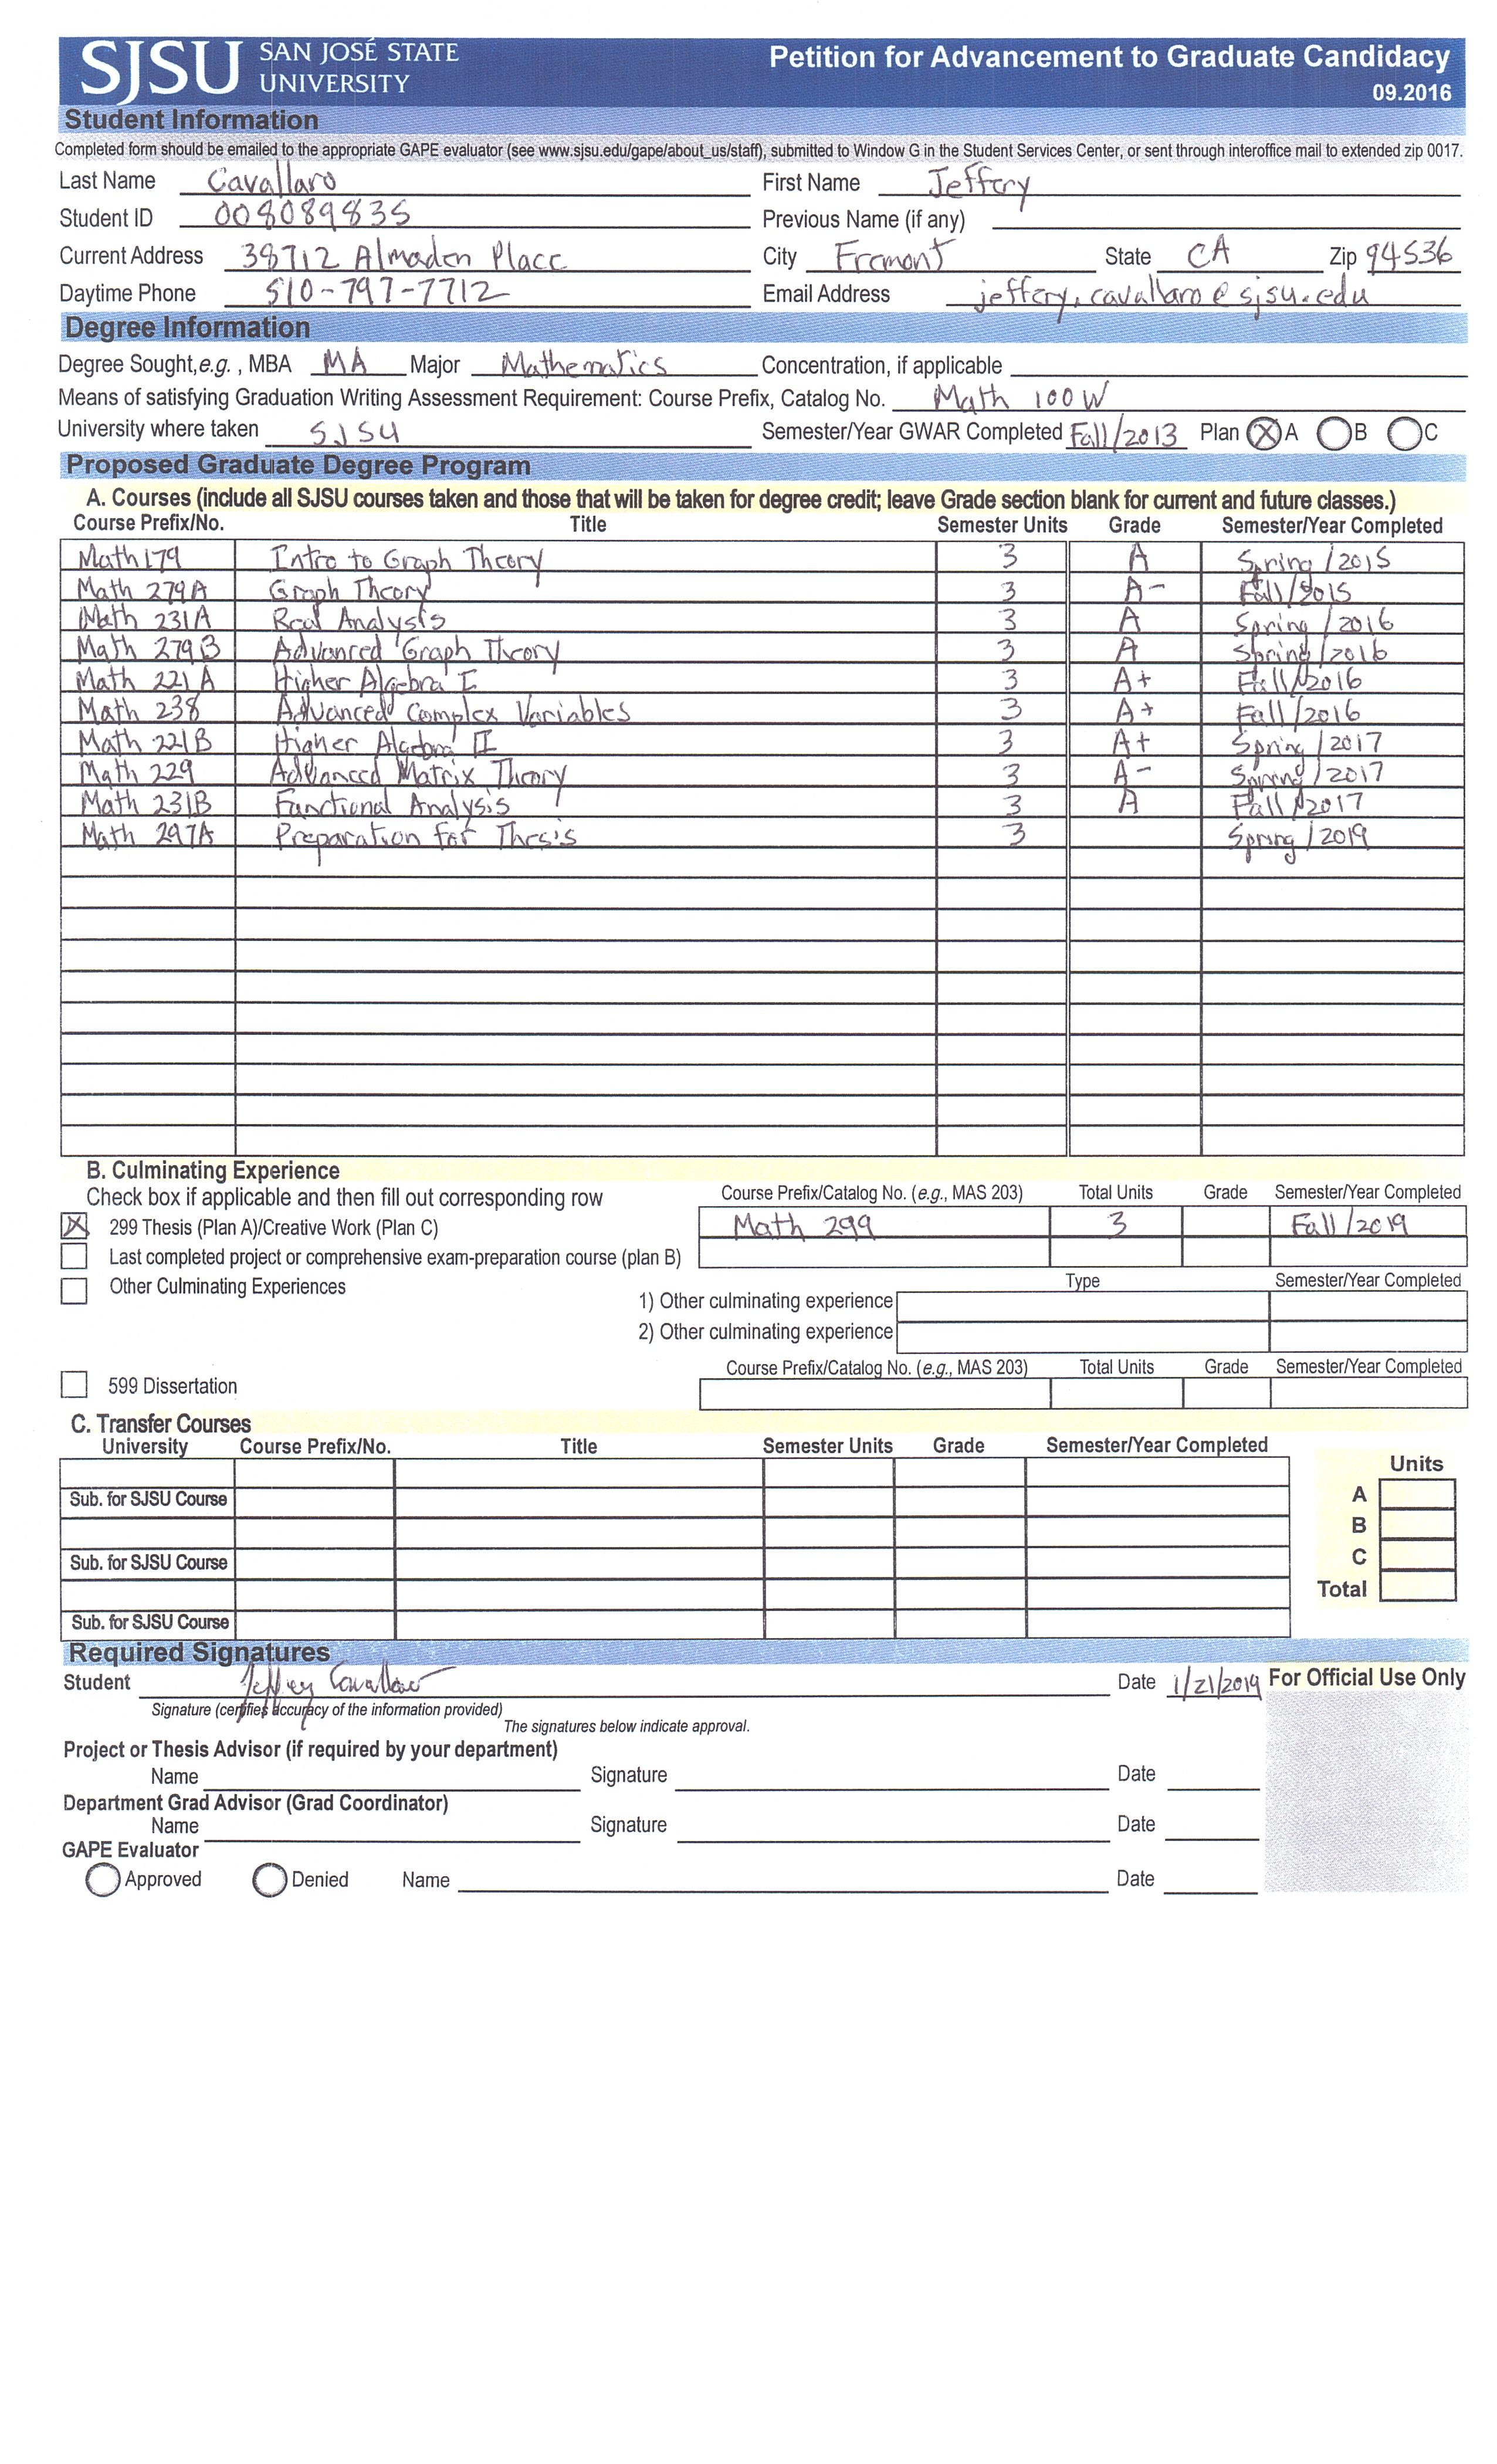
\includegraphics[scale=0.9]{candidacy.jpg}

\end{document}
